\section{Theory}

Our dataset consists of images.  One could use each individual pixel as an individual input feature, but that loses any relative spacial locality information between pixels, and is therefore prone to errors due to location in the image of the object to be identified \cite{lecun1998gradient}.  For example, if we want to identify if an image has a circle or not, looking at a set of pixels without knowing where they are located relative to eachother cannot be done in general.

For handwriting recognition, there are some features that some people have tried to extract to use in a learning algorithm.  These include aspect ratio, percent of thresholded pixels above the horizontal half plane, percent of thresholded pixels to the right of the vertical half plane, and so forth \cite{web:wikihandwritfeat}.  It is unknown if these features will be sufficient to classify the characters.

\subsection{Convolutional Neural Networks}

Early on in the project, we received a recommendation to use Convolutional Neural Networks (CNNs).  CNNs have been shown to be very effective in image recognition \cite{korekado2003convolutional} \cite{ciresan2012multi}.  One significant advantage of CNNs is the ability to make the representation \emph{invariant} to small translations of the input, such as for image recognition tasks \cite{Bengio-et-al-2015-Book}.  Another useful aspect of CNNs are their ability to automate feature identification and extraction \cite{Bengio-et-al-2015-Book}.

\begin{figure}[ht]
  \centering
  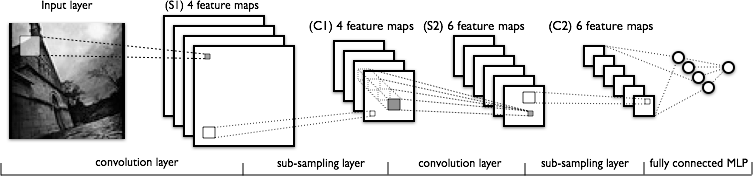
\includegraphics[width=\textwidth]{images/mylenet.png}
  \caption{
    Convolution and pooling layers that make up a CNN followed by a
    fully-connected Multi-layered Perceptron (MLP).
    (from \cite{Bengio-et-al-2015-Book})
    }
  \label{fig:convnet}
\end{figure}

CNNs are an example of multi-layered neural networks.  As can be seen in Figure~\ref{fig:convnet}, CNNs have convolution layers and sub-sampling layers, also known as pooling layers.  The convolution layer uses multiple weight matrices to generate other images.  These are then pooled in order to reduce the dimensionality while at the same time introducing non-linearities.  The type of non-linearity depends on the function used in the pooling layer, such as a max function over a $4 \times 4$ region.  We have a loss function at the end of the neural pipeline, and train the previous layers by performing back-propagation.  This back-propagation is simply gradient descent over all of the weight vectors in the whole network (by doing chain rule).

We studied some example code of CNN on \url{deeplearning.net}.   By reading their code, we made two interesting observations.
\begin{description}
  \item[Kernels]
    Multiple weight filters are generated at each convolution layer.  How do they not converge to the same weight vector?  We believe this has to do with the space not being convex and having multiple local minima, because of the introduced non-linearities at each layer.  We initialize the weight vectors with random values and hope that they find different local minima.  We treated this value as a hyper-parameter.  We suspect that having this value too high will both cause a significant increase in running time and cause the resultant classifier to overfit.
  \item[Weight bounds]
    The initialization of the weight bounds seemed to be determined
\end{description}

\subsection{Theano}

We were pointed by Dustin Webb to the Theano python module for implementation of CNNs.  Theano takes mathematical expressions and compiles them into C++ to make for a robust and efficient framework \cite{bergstra+al:2010-scipy}.  Theano was something completely new to us.  It uses symbolic expressions that can be compounded together.  You can define a loss function and have Theano symbolically generate the gradient for use in stochastic gradient descent.

\subsection{Linear Classifiers}

Even though we chose to use CNNs, we decided to first employ the linear classifiers we learned in class for comparison and to learn how to use Theano.  We chose to use Perceptron, Averaged Perceptron, SVM, and Logistic Regression.  These all can be implemented using stochastic gradient descent even though Perceptron is usually not directly implemented in that way.
